\subsection{Minimization reallocates transcription toward translation at the expense of central metabolism}

Minimization removed not only genes but a share of the expression budget.
Of the 911 \syn~loci, 418 are absent from \syna (382 protein-coding, 33 pseudogenes, 3 structural RNAs), together carrying 21.8\% of the messenger-RNA pool and 22.3\% of the proteome in \syn.
Nearly half the genes thus held only about a fifth of the output, so the removed loci were well below average in expression, and their most transcribed members are all dispensable in rich medium: the yeast-vector marker \gene{lacZ}{0915}, the pyruvate-dehydrogenase subunits \gene{pdhA}{0225} and \gene{pdhB}{0226}, and alanine dehydrogenase \gene{ald}{0059}~\cite{breuer_essential_2019}.
Although this frees a fifth of the messenger-RNA pool, central-carbon metabolism and the other enzymatic subsystems command a smaller share of it in \syna, not a larger one (central-carbon 17.0\% to 10.7\%); most of the freed capacity is instead reallocated to translation (53.1\% to 64.9\%; Fig.~\ref{fig:reduction_omics}a; comparisons are mean-normalized to the retained pool, \hyperref[method:reduction-normalization]{Methods}).

This reallocation rode on a globally conserved expression hierarchy (Fig.~\ref{fig:reduction_omics}b).
Per-gene relative transcript levels in \syn~and \syna~correlated at Pearson $r = 0.84$ on $\log_{10}$ relative TPM (each gene's TPM relative to the average gene TPM, which counteracts the different gene numbers of the two cells; $n = 443$ protein-coding genes), and the proteome to a similar degree ($r = 0.87$ on $\log_{10}$ relative iPM, its protein analogue, $n = 423$), so the ancestral program was inherited largely intact at both layers.
Yet two thirds of the retained genes (66\%) fell in relative transcript level, the arithmetic shadow of the freed capacity being taken up by a few large risers rather than spread across functions.
Those risers were overwhelmingly ribosomal proteins (\gene{rpsK}{0646}, \gene{rplO}{0653}, \gene{rplX}{0660}, \gene{rplN}{0661}, each gaining 4.3 to 6.0 relative units), and most of the gain issued from a single 21-gene ribosomal-protein operon that alone supplies about a third of the \syna~coding messenger-RNA pool (Fig.~\ref{fig:reduction_omics}d).
The rise was selective rather than uniform for all 51 ribosomal proteins: the fusion-affected \gene{rpsT}{0082} and \gene{rpsO}{0294} instead collapsed (Fig.~\ref{fig:reduction_operons}), and three structurally intact r-proteins (\gene{rpmF}{0526}, \gene{rpmE}{0137}, \gene{rpsU}{0482}) fell sharply in transcript despite unchanged context.

Two protein-only gene-expression machines moved in opposite directions, estimated from their limiting subunit (Fig.~\ref{fig:reduction_omics}c).
Core RNA polymerase (minimum of \textit{rpoA}/2, \textit{rpoC}, \textit{rpoB}) fell to a fold change of 0.65 in transcript and 0.79 in protein (35\% and 21\% reductions), whereas the RNase~Y-based degradosome~\cite{redko_minimal_2013} (minimum of \textit{rny}, \textit{rnjA}, \textit{yhaM}\,+\,\textit{rnr}) rose to 1.68 and 1.36 (68\% and 36\% increases).
Lower transcription capacity together with higher RNA-turnover capacity is coherent with \syna's longer cell cycle, roughly 105~min against 60~min for \syn~\cite{pelletier_genetic_2021}.

Central-carbon metabolism declined in concert at both layers (Fig.~\ref{fig:reduction_omics}c).
Central Carbon Metabolism as a whole fell from 17.0\% to 10.7\% of the retained pool (median fold change 0.66, two-sided Mann--Whitney $p = 1.3\times10^{-3}$), with smaller losses in Membrane Transport (0.80, $p = 0.016$) and Transcription (0.55, $p = 0.040$).
In glycolysis \gene{eno}{0213}, \gene{pgk}{0606}, and \gene{pyk}{0221} fell to transcript/protein fold changes of 0.37/0.38, 0.35/0.44, and 0.51/0.34; the pyruvate-dehydrogenase E1 subunits \gene{pdhA}{0225} and \gene{pdhB}{0226} were deleted outright while the retained E2 \gene{pdhC}{0227} dropped to 0.45/0.34; and the acetate and lactate steps \gene{pta}{0229}, \gene{ackA}{0230}, and \gene{ldh}{0475} fell to 0.27/0.26, 0.19/0.44, and 0.66/0.70.
Part of this decline is the promoter-loss decapitation of the pyruvate-dehydrogenase and glucose-PTS operons shown earlier (Fig.~\ref{fig:reduction_operons}), the rest the pool-level downshift onto which it is superimposed.
This concerted downgrade predicts lower ATP and GTP output in \syna, a prediction awaiting an explicit metabolic-flux comparison.

The reallocation toward translation was dominated by this one transcription unit (Fig.~\ref{fig:reduction_omics}d).
The $\sim$11~kb ribosomal-protein operon \locus{0652}--\locus{0672}, a 21-gene polycistron from one promoter (a canonical \texttt{TANAAT} $-10$ box, \texttt{TAGAAT}) with no predicted internal terminator, rose from 12\% of the \syn~coding messenger-RNA pool to 34\% in \syna, so over a third of all coding transcription in the minimal cell issued from this one operon.
Full-length $\sim$11~kb reads were rare at the read-length limit, but continuous coverage with no internal terminator marked it as one unit, while a steep 5$'$ polarity gradient and a sharp depth step indicated internal endonucleolytic processing.
The flanking deletions, which removed \gene{dhaK}{0673} through \locus{0677}, brought a co-directional four-tRNA operon (\locus{0678}--\locus{0681}) to within 772~bp of its start, against 7{,}193~bp in \syn, yet the operon's own promoter was retained 179~bp from the nearest deletion.
Despite this adjacency the two were not co-transcribed (no \syna~direct ONT RNA read spanned the junction; intervening short-read coverage 1.2\% of the flanking depth; Fig.~\ref{fig:reduction_omics}d), so the operon's dominance rested on its own retained promoter and the pool-level reallocation, not on read-through from the relocated tRNA genes.

% Paragraph order (2026-07 restructure): P1 removal + pool composition (a) / P2 conserved-but-down + translation rise (b) / P3 machines (c) + central-carbon enzymes (c) / P4 the giant rPtn operon + its swapped upstream neighbour (d). L6.5 ATP/GTP flux stays text-only (needs a metabolic-flux model). Panel d MERGES old d (operon structure) + old e (tRNA junction) into one transcript-axis figure: Syn1 genes+depth over Syn3A genes+depth, aligned on the rpsJ/0672 5' end (R6_figure_panels.py::panel_d). The two P4 paragraphs now both point at (d).

\begin{figure}[H]
    \centering
    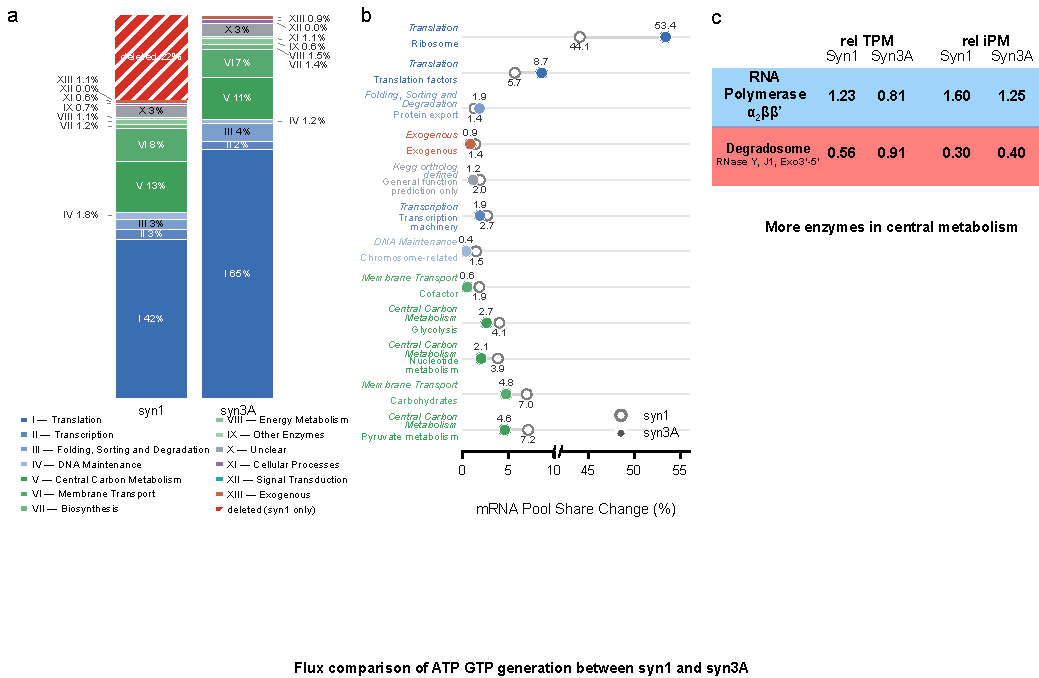
\includegraphics[scale=1]{figures/reduction_omics.pdf}% born-at-size: native 177.8 mm, fits the 180 mm text block
    \caption{\textbf{The \syna~ mRNA pool and proteome reallocate towards translation machinery, especially the 21-gene ribosomal protein operon.}
    (a) Composition of the retained messenger-RNA pool by Secondary function in \syn~and \syna, deletion-corrected.
    (b) Retained-pool mRNA fold change (\syna/\syn) versus absolute change, the 51 ribosomal proteins highlighted; inset, the \syn-vs-\syna~relative-mRNA correlation ($r = 0.84$) in which two thirds of genes fall below the diagonal.
    (c) mRNA and protein fold changes of RNA polymerase, the degradosome, and the central-carbon enzymes.
    (d) The 21-gene $\sim$11~kb ribosomal-protein operon (\gene{rpsJ}{0672}$\rightarrow$\gene{secY}{0652}, minus strand) and its upstream neighbourhood in \syn~and \syna, aligned on the shared operon 5$'$ end (transcription start; gene tracks with Illumina depth, $\times$ genome-mean).}
    % The retained operon is identical between the two cells and reads as a single polycistron at high 5$'$ depth with internal processing steps; only the upstream neighbour changed, from \gene{dhaK}{0673} in \syn~to the four-tRNA operon (\locus{0678}--\locus{0681}) pulled to within $\sim$770~bp in \syna, with no read-through across the silent inter-operon gap.}
    \label{fig:reduction_omics}
\end{figure}
